\section{Serial latency, quality, and energy}
\label{sec:wins}

\paragraph{Direct latency comparison.}
In the repeated BGL runs at batch size one, AR-30B has median latency
\arMedian\,ms (95\% bootstrap CI [\arCiLo, \arCiHi]; 900 events
pooled across seeds 42, 137, and 314). DG has median \dgMedian\,ms
(CI [\dgCiLo, \dgCiHi]; 2,000 events). The ratio of these medians
is approximately $2.4\times$. Bootstrap intervals use 10,000 event-level
resamples. The AR seed-median CV is \seedCV\%, describing repeatability
across these three runs rather than uncertainty across hardware or workloads.

A two-sided permutation test of the absolute median difference observed
no equally or more extreme result in 100,000 shuffles. The finite-sample
Monte Carlo estimate $(0+1)/(100000+1)$ is approximately $10^{-5}$;
we do not interpret the stored zero exceedance fraction as a zero
probability. This unpaired test treats event timings as exchangeable and
does not control run-level differences or temporal dependence. The
observed latency gap is large, but its interval is conditional on these
measurement assumptions.

\begin{figure}[ht!]
\centering
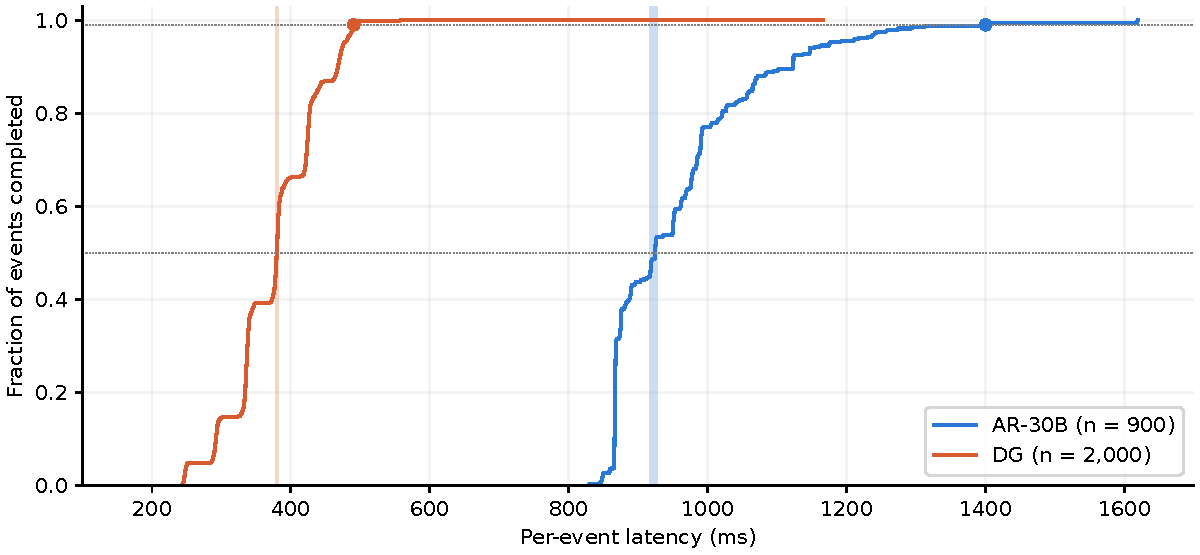
\includegraphics[width=0.88\linewidth]{figures/fig12_v8.pdf}
\caption{Empirical cumulative distributions of saved BGL event latencies:
AR-30B, 900 events across three seeds; DG, 2,000 events. Shaded bands
mark bootstrap 95\% intervals for each median. DG has lower median and
p99 latency, despite a larger coefficient of variation and max/median
ratio. These are service times, excluding arrival-queue delay.}
\label{fig:distributions}
\end{figure}

\paragraph{Quality is a separate constraint.}
The serial-sweep AR-30B 9-field F1 is 0.870. The earlier paired quality
analysis compared DG with dense AR-3B (\arThreeBFnine), not AR-30B.
It therefore cannot establish quality equivalence for the primary latency
pair. Faster service may be useful when DG meets the application's quality
threshold, but the current evidence does not establish a $2.4\times$
speedup at matched quality. This distinction also applies to the
throughput and cost comparisons.

\paragraph{Output budget is not generated length.}
Table~\ref{tab:niche} retains the original serial-sweep means so that
the fitted cost model can be traced to its source. These are different
runs and a different summary statistic from the repeated medians above.
AR emits approximately 126 tokens when its budget is sufficient and
then stops. Increasing the budget from 256 to 1024 does not lengthen
its output. By contrast, charging DG for all canvases permitted by the
budget increases its predicted cost. The resulting ratio is a
\emph{budget-accounting comparison}, not an observed long-output task
speedup.

\begin{table}[ht]
\centering
\caption{AR serial-sweep mean service time ($n{=}300$ per cell) versus
DG full-canvas cost from Eq.~\ref{eq:dg}. DG values are predictions
from measured canvas costs, not paired event means. The AR rows at
budgets 32 and 128 are output-limited; a 48-token cost crossover does
not imply valid extraction at that budget.}
\label{tab:niche}
\begin{tabular}{@{}rrrrr@{}}
\toprule
Budget $B$ & AR mean (ms) & AR mean tokens & DG model (ms) & AR/DG \\
\midrule
32 & 265 & 32 & 379 & $0.7\times$ \\
128 & 907 & 121 & 379 & $2.4\times$ \\
256 & 945 & 126 & 379 & $2.5\times$ \\
512 & 945 & 126 & 498 & $1.9\times$ \\
1024 & 945 & 126 & 737 & $1.3\times$ \\
\bottomrule
\end{tabular}
\end{table}

Extending this accounting to a 2048-token DG budget reverses the
ratio to approximately $0.8\times$: AR has already stopped while DG
is charged for eight canvases. Conversely, a task that actually requires
long AR output could widen DG's advantage. That case requires a new
natural-output evaluation; Appendix~\ref{app:forced} labels the
available calculation as a projection.

\paragraph{Throughput is not response latency.}
The AR-30B batch experiment completes 300 requests in 12.08\,s,
corresponding to 40.3\,ms per event when total elapsed time is divided
by batch size. Individual requests do not therefore return in 40.3\,ms.
That inverse-throughput measure must not be substituted for serial
response time. It underlies the approximately $25\times$ batching
multiplier in \S\ref{sec:limits}.

\paragraph{Energy.}
The saved AR-30B serial power run reports \arEnergy\,J per event
above idle, compared with \dgEnergy\,J for DG in a separate run.
The descriptive ratio is approximately $40\times$. The AR run records
223.0\,W mean board power, 49.73\,W idle, and 288.249\,s for 300
events; the DG run records 63.4\,W, 52.6\,W idle, and 38.57\,s for
100 events. Thus the direction is consistent with both lower DG net
power and shorter service time in these runs.

These measurements use different idle baselines, sample counts, and
power-sampling rates, with only 39 power samples in the DG run.
They do not isolate an architectural cause, and the idle-subtracted
ratio is sensitive to the small DG difference between active and idle
power. We treat it as preliminary board-energy evidence, not an
end-to-end energy-efficiency ratio or a controlled deployment-cost result.
